\documentclass{beamer}

\usepackage{threeparttable}

\newcommand{\eps}{\epsilon}
\newcommand{\var}{{\rm var}}
\newcommand{\cov}{{\rm cov}}
\newcommand{\nid}{{\rm NID}}
\newcommand{\diag}{{\rm diag}}
\newcommand{\E}{{\mathrm E}}
\newcommand{\R}{{\mathrm R}}
\newcommand{\RD}{{\tilde{\mathrm R}}}
\newcommand{\Q}{{\mathrm Q}}
\newcommand{\U}{{\mathrm U}}
\newcommand{\Ex}{{\cal E}}
\newcommand{\cor}{\mathrm{cor}}
\newcommand{\tr}{\mathrm{tr}}
\newcommand{\e}{\mathrm{e}}
\newcommand{\de}{\mathrm{d}}
\newcommand{\p}{\mathrm{P}}
\newcommand{\Ln}{\mathrm{Ln}}
\newcommand{\sign}{\mathrm{sign}}

\newcommand{\ra}{\varrho}

\newcommand{\minn}{\mathrm{min}_n}
\newcommand{\maxn}{\mathrm{max}_n}


\newcommand{\cq}{\ ,\quad }
\newcommand{\qq}{\quad \Rightarrow \quad}
\newcommand{\oq}{\quad \Leftarrow \quad}
\newcommand{\eq}{\quad \Leftrightarrow \quad}



\newcommand{\ppo}[1]{|{#1}|^+}

\newcommand{\ssection}[1]{%
  \section[#1]{\textbf{\uppercase{#1}}}}
\newcommand{\ssubsection}[1]{%
  \subsection[#1]{\normalfont\textbf{#1}}}


%\renewcommand{\labelenumi}{(\roman{enumi})}

\newcommand{\eref}[1]{(\ref{#1})}
\newcommand{\fref}[1]{Figure \ref{#1}}
\newcommand{\sref}[1]{\S\ref{#1}}
\newcommand{\tref}[1]{Table \ref{#1}}
\newcommand{\aref}[1]{\ref{#1}}



\newcommand{\bi}{\begin{itemize}}
\renewcommand{\i}{\item}
\newcommand{\ei}{\end{itemize}}



\newcommand{\es}{{\mathrm{ES}}}
\newcommand{\ses}{{\mathrm{SES}}}
\newcommand{\sr}{{\mathrm{SR}}}

\bibliographystyle{chicago}

% \usepackage{beamerthemesplit} // Activate for custom appearance

\title{Capital Shortfall in Banks and Stress testing}
\author{Piet de Jong, Geoff Loudon, Weihao Choo}
\date{\today}

\begin{document}

\frame{\titlepage}

\frame{\frametitle{Outline of presentation}
\bi
\i   Capital shortfall \framebox{Brownlees \& Engle (2015)}
\i   Future (1 month's time) capital shortfall \framebox{$S$}
\i   Example:  CBA return  \& market return
\i   Stress testing capital shortfall -- scenarios \framebox{$\omega$}
\i   Stress testing -- ``theory" --  stress function \framebox{$\psi(\omega)$}
\i   Proposed definition of "stress"  \framebox{$\psi_S$} ... $\psi$--risk in/on $S$
\i   Properties/features/estimating  \framebox{$\psi_S$}
\i   Baseline risk (BASRISK), $\psi$--risk (PSIRISK)
\i   Detailed look at 8 Australian banks 2003-2015 
\i   Formalisation of risk weighted assets methodology
\ei
}

\frame{\frametitle{What's new in this paper?}
\bi
\i  Build on techniques of Brownlees \& Engle (2015)
\bi
\i   Capital shortfall -- volatility lab
\i   GARCH-DCC methodology to model same
\i   Systemic stress measurement
\ei
\i  Development of  \framebox{statistical ``stress" methodology}
\bi
\i  Can be applied to any joint distributional framework
\i  Based on \framebox{stress function}
\i  Based on \framebox{stressed} probabilities and conditional expectation
\i  Distinguishes between \framebox{background} and \framebox{systemic} stress
\i  Appropriate quantitative definition of \framebox{systemic} stress
\ei
\i  Appropriate \framebox{aggregation} of stress and stress \framebox{contributions}
\i  Application to 8 Australian banks
\i  Comparison to asset risk weighting methodology
\i \framebox{Not done}:     
\bi
\i  Other Aust financial institution (insurance, bldg societies, etc)
\i EURO or US banks
\ei
\ei
}


\frame{\frametitle{Capital Shortfall -- Brownlees \& Engle (2015)}
$$
S= k (d+w)-w = k d\left(1-\frac{1-k}{kL}\right)
$$
\bi
\i  $d$ is debt, $w$ is equity, $d+w$  assets, $L\equiv \frac{d}{w}$ is the {\bf leverage}
\i  $k$ is the {\bf prudential fraction} -- often around 8\%, capturing market, credit, insurance, operational and other risks
\i  $S$ is amount ($\pm$)  to maintain {\bf solvency}.  $S<0$  indicates capital surplus
\i {\bf Definition of $S$ is  simplistic} ... 
\bi
\i  Maybe additional adjustments  relating to intangible assets and liability surpluses
\i Firms usually need to maintain an equity buffer above regulatory capital requirement and hence the true capital shortfall is higher
\ei
\i \framebox{$S=kd(1-\e^{-\ell})$} where $\ell=\ln\left(\frac{kL}{1-k}\right) = \mathrm{logit}(k) + \ln(L)$
\bi
\i   {\bf $\ell$ is the adjusted log--leverage}:  $\ell>0$  implies $S>0$
\ei
\ei
}

\frame{\frametitle{Australian Banks:  $w$ and $\ell$}
\begin{figure}[htbp]
\begin{center}
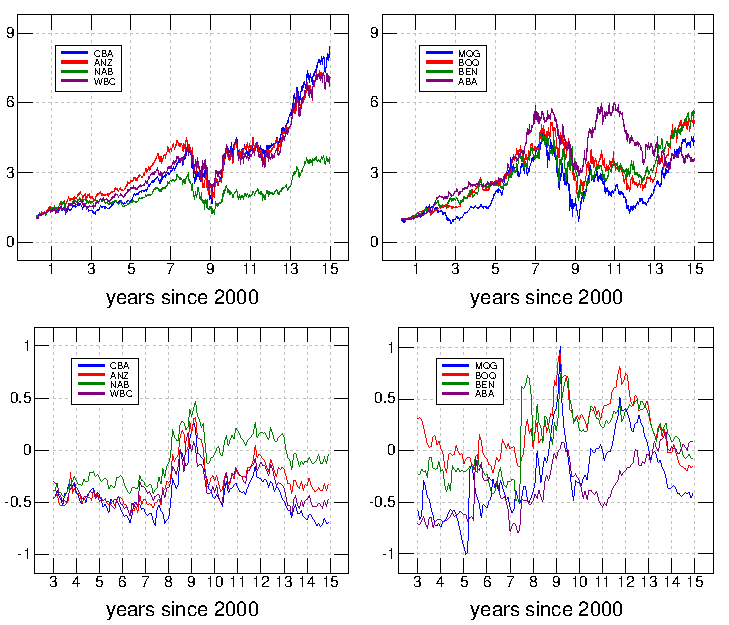
\includegraphics[width=7.5cm]{figures/prices2.pdf}
\caption{Daily stock  prices of four major (top left panel) and four minor (top right panel) Australian banks from early 2000 through to the end of 2014.  Price series normalised to start at 1. Bottom panels are adjusted log--leverages at start of every month from 2003 onwards.}
\label{prices}
\end{center}
\end{figure}
\bi
\i  Debt $d$ smooth step function
\i  In calculations below based on $k=8\%$  (Basel fraction)
\ei
}


\frame{\frametitle{Future capital shortfall}
  Interested in  capital shortfall in,  say, \framebox{1 month's time}
  $$
  S\equiv k d\left(1-\frac{1-k}{kL\e^{-r}}\right) = kd(1-\e^{r-\ell})
  $$
\bi
\i Assumes debt $d$ does \framebox{not} change over the month
\i  $r$ is the return on on equity:   $\e^rw$ equity in one month's time
\i $L$ is the current leverage:  $L\e^{-r}$ future leverage
\i $\ell$ is the (current) adjusted log--leverage.   If $r<\ell$ then $S>0$
\i  Interested in  $\E(S|\omega)$ under \framebox{adverse} scenarios $\omega$
\i  $\E(S|\omega)-\E(S)$ is the $\uparrow$ shortfall ``risk"  of  $\omega$
\bi
\i  What are  appropriate adverse scenarios $\omega$?
\i  How to model/calculate $\E(S|\omega)$? 
\ei
\ei
}

\frame{\frametitle{Example -- adverse scenario is market downturn}
\begin{figure}[htbp]
\begin{center}
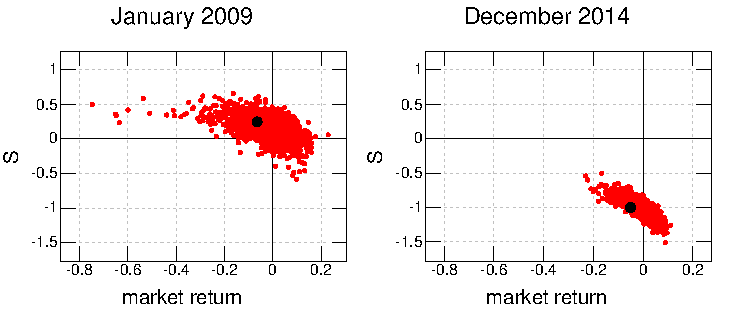
\includegraphics[width=9cm]{figures/figCBA.pdf}
\caption{Forecast $(\omega,S)$ distribution where $\omega$ is one month forward market return and $S$ is CBA shortfall with $k=0.08$.  Distribution derived from $N=6000$ simulations based on GARCH--DCC model.  Axes in both panels are same scale.  Black dots indicate actual outcomes.}
\label{figCBA}
\end{center}
\end{figure}
\bi
\i  Generally $\uparrow$ market return  leads to $\downarrow S$
\i  Radically different risk of shortfall under market scenarios
\i  How to ``stress test"?
\ei
}

\frame{\frametitle{``What if" analysis:  Stress testing}
\bi 
\i {\bf Response}: $S$ -- e.g. capital shortfall in a bank
\i {\bf Scenario}: $\omega$  -- e.g. drop in housing prices
   \bi\i Scenario is {\bf systemic} since expected to effect many banks
       \i e.g. $\omega$ is 25\% reduction in  house prices
       \i $\omega$ is usually a  SINGLE scenario
    \ei
\i  {\bf Real world probability}: $f(\omega)$ known or unknown
\i {\bf  Baseline risk (BASRISK)}: $\E(S)$
\i  {\bf Stress function}: $\psi(\omega)=1/f(\omega)$, for given $\omega$, 0 otherwise
\i  {\bf Stressed probabilities}: $\tilde f(\omega) = \psi(\omega)f(\omega) = 1$, 0 otherwise
\i  {\bf Stressed risk}: $\widetilde\E(S) = \E(S|\omega)$
\i {\bf $\psi$--risk (PSIRISK) in $S$}: $\psi_S = \widetilde\E(S)-\E(S)$
\i  {\bf Modelling -- Computation}:   Spreadsheet to see effect on banks balance sheet and in particular on capital shortfall $S$.
\ei   
}




\frame{\frametitle{Stress testing:  proposed   ``framework/theory"}
\bi
\i   {\bf Response} random variable \framebox{$S$} 
\bi \i E.g. $S$ is the future capital shortfall of a bank or group of banks.  Or  indicator of a positive shortfall. \ei
\i {\bf Scenarios}  \framebox{$\omega$}. Mutually exclusive and exhaustive
\bi 
\i  best thought of as (generated by) one or more variables  ({\bf stressors}?)
\i  {\bf systemic} if they have impact on many response variables
\ei

\i {\bf Real world probabilities}:  \framebox{$f(\omega)$} 
\i  {\bf Baseline risk}: \framebox{$\E(S)\equiv\sum_\omega f(\omega) \E(S|\omega)$} 
\bi      \i If $\omega$  continuous then $f(\omega)$ is  a density, expectation an integral \ei
\i {\bf Stress function}: \framebox{$\psi(\omega)\ge 0$  with  $\E(\psi)=1$}
\bi
\i $\psi$ is  often subjective
\i $\psi$ can be regarded as a random variable on space of scenarios
\ei
\i {\bf Stressed probabilities}: {\small\framebox{$\tilde f(\omega)\equiv \psi(\omega)f(\omega)$}}
\bi \i $\psi(\omega)>1$ implies scenario $\omega$ is amplified  in importance \ei 
\i {\bf Stressed risk}:
\framebox{$ \widetilde \E(S) \equiv \E(\psi S)= \sum_\omega \tilde f(\omega)\E(S|\omega)$}   
\i {\bf $\psi$--risk} in $S$: \framebox{$\psi_S\equiv \widetilde\E(S)-\E(S)$}
\bi \i If $\psi(\omega)$ is constant then $\psi_S=0$ \ei
\ei
}

\frame{\frametitle{Example (1)}
  \bi
  \i  {\bf Response}:  $S$ -- capital shortfall in a bank
  \i  {\bf Scenario(s)}: $20\% $  housing market ``correction" 
  \bi
  \i Scenario is {\bf systemic} since expected to effect many banks
  \ei
  \i  {\bf Real world probabilities}: $f(-20\%)=?$
  \i  {\bf Stress function}: $\psi(-20\%)=1/f(-20\%)$, 0 otherwise
  \bi
  \i   completely emphasises -20\% outcome, \framebox{ignores all others}
  \i  $\E(\psi)=1$; direct calculation
  \ei 
  \i  {\bf Stressed probabilities}: $\tilde f(\omega) \equiv \psi(\omega)f(\omega) = \framebox{1 or 0}$
  \i {\bf Stressed risk}:   $\widetilde\E(S) \equiv \E(S|-20\%)$
  \i {\bf $\psi$--risk in $S$}: \framebox{$\psi_S \equiv \widetilde\E(S)-\E(S)$} ... ``elevated risk due to $\psi$"
  \i {\bf Computations}:   Spreadsheet or similar
  \i {\bf Criticisms}:   One scenario emphasised -- \framebox{all others ignored}
  \ei
}



\frame{\frametitle{Example (2) ... more realistic}
  \bi
  \i  {\bf Response}:  $S$, capital shortfall in a bank
  \i  {\bf Scenarios}: $0\le \omega\le 1 $   {\bf percentile} housing market downturn
  \bi
  \i Scenario is {\bf systemic} since expected to effect many banks
  \ei
  \i  {\bf Real world probabilities}: \framebox{$f(\omega)=1$}, the uniform density
  \i  {\bf Stress function}: \framebox{$\psi(\omega)=n(1-\omega)^{n-1}$}
  \bi
  \i   emphasises lower (bad) percentiles ; downplays others
  \i  $\E(\psi)=1$; direct calculation
  \ei 
  \i  {\bf Stressed probabilities}: $\tilde f(\omega) \equiv \psi(\omega)f(\omega) = \framebox{$n(1-\omega)^{n-1}$}$
  \bi
  \i  density of the {\bf worst percentile in $n$ independent trials}
  \ei 
  \i {\bf Stressed expectation}:   $\widetilde\E(S) \equiv \int_0^1\tilde f(\omega)\E(S|\omega)\de\omega=\E(S|\Omega)$
  \bi
  \i $\Omega$ is the event ``worst market outcome in $n$ months"
  \ei
  \i {\bf $\psi$--risk}: \framebox{$\psi_S \equiv \widetilde\E(S)-\E(S)$} ... ``elevated risk due to $\psi$"
  \ei
}


\frame{\frametitle{Example (3), (4), ...}
\bi
\i   Other response variables \framebox{$S$}
\i   Other scenario spaces/stressors \framebox{$\omega$}
\bi
\i   Oil prices fall ...,  Metal prices fall ...., Interest rates rise ... 
  terrorist attack ..., bank X collapses ..., Grexit ...
\i   Combinations (product spaces $\bigotimes$) of the above
\i   \framebox{percentile outcome} of a variable
\ei
\i   Real world probabilities \framebox{$f(\omega)$}
\bi \i Perhaps from a model 
\i Copulas useful if $\omega$ percentile and $\bigotimes$
\ei
\i   Stress function \framebox{$\psi(\omega)$}
\bi
\i Model $f(S,\omega)=f(\omega)f(S|\omega)$ and stress $f(\omega)$
\i If \framebox{$\omega$} percentile outcome  of a variable then $f(\omega)=1$ and then can perform \framebox{percentile} stressing
\ei
\ei
}

\frame{\frametitle{Understanding $\psi$--risk  (PSIRISK)}
$$
\widetilde\E(S) \equiv \sum_\omega \tilde f(\omega)\E(S|\omega) = \sum_\omega \psi(\omega)f(\omega)\E(S|\omega) 
$$$$
= \E(S\psi)=\E(S)\E(\psi) +\cov(S,\psi) =  \E(S) + \cov(S,\psi)
$$
\bi
\i \framebox{BASRISK$\equiv\E(S)$} ... baseline risk not allowing for $\psi$
\i \framebox{PSIRISK$\equiv\psi_S\equiv\cov(S,\psi)
 =\widetilde\E(S)-\E(S)$} ... extra risk
\bi
\i   $\psi_S$ large if $S$ and $\psi$ have large covariance
\i   $\cov$ is linear in $S$ and $\psi$ ... even if components  dependent
\i   $\cov(S,\psi)=\cov\{\E(S|\psi),\psi\}$
\ei
\i \framebox{PSIVOL=$\sigma_\psi\equiv\sqrt{\psi_\psi}$} ... $\psi$--volatility
\bi
\i $\psi(\omega)=1/f(\omega)$, 0 implies $\sigma_\psi=\e^{-\mathrm{logit}\{f(\omega)\}/2}$
\i unlikely scenario, $f(\omega)\approx 0$, implies huge PSIVOL
\ei
\i \framebox{$\E(S|\psi=x) \approx   \E(S) + \frac{\psi_S}{\sigma^2_\psi}(x-1)=\mathrm{BASRISK}+\frac{\mathrm{PSIRISK}}{\mathrm{PSIVOL}} z_x$}
\ei
}

\frame{\frametitle{Understanding PSIRISK (cont.)}
$$
\framebox{$-1\le\frac{\widetilde\E(S)-\E(S)}{\sigma_S\sigma_\psi}= \frac{\psi_S}{\sigma_S\sigma_\psi}
=\frac{\cov(S,\psi)}{\sqrt{\cov(S)\cov(\psi)}}\le 1$}
$$
\bi
\i {\bf Stress ``z--score"}: 
\framebox{$z\equiv \frac{\widetilde\E(S)-\E(S)}{\sigma_S}=\frac{\psi_S}{\sigma_S}=\sigma_\psi\cor(S,\psi)$}
\bi
\i ``connection" between $S$ and $\psi$  multiplied by $\psi$--vol
\i not affected by $S$ units of (linear) measurement
\i $|z|\le \sigma_\psi$
\i perhaps $z>2$ regarded as ``stressful" 
\ei
\i {\bf Standardised  $\psi$--risk}:
\framebox{$\psi_S^* \equiv \frac{\psi_S}{\sigma_\psi}=\frac{\widetilde\E(S)-\E(S)}{\sigma_\psi}=\sigma_S\cor(S,\psi)$}
\bi
\i  ``connection" between S and  $\psi$ multiplied by $S$--volatility
\i facilitates comparison across different stressors $\psi$
\i not affected by $\psi$-vol
\i $\E(S|\psi=x) \approx \E(S) +\psi_S^*\times\frac{x-1}{\sigma_\psi}$ so $\psi_S^*$ is std reg coef $S$ on $\psi$
\i $\frac{\E(S|\psi=x) - \E(S)}{\sigma_S} \approx \cor(S,\psi)\times \frac{x-1}{\sigma_\psi}$
\ei
\ei
}



\frame{\frametitle{BASRISK and PSIRISK computations}
\bi
\i Suppose   a model leading to $f(S,\omega)\equiv f(\omega)f(S|\omega)$
\bi
\i Repeat $N$ times:   $\omega\sim f(\omega)$ and $S(\omega)\sim f(S|\omega)$ then
\i  BASRISK= Baseline Risk = $\E(S)\approx \frac{1}{N}\sum_\omega S(\omega)$ 
\i PSIRISK$=\psi_S=\widetilde\E(S)-\E(S) \approx\frac{1}{N}\sum_\omega \{\psi(\omega)-1\}S(\omega)$
\ei
\i  Alternatively construct estimates of $\E(S)$ and $\E(S|\psi)$
\bi
\i   Perhaps via spreadsheet
\i  $\psi_S = \cov\{\E(S|\psi),\psi\}$
\ei
\i  If $\psi(\omega)$ is based on percentile of $\omega$ then
\bi
\i  $\psi(\omega) = \phi\left\{F(\omega)\right\}$ with $F(\omega)\approx\mathrm{rank(\omega)}/N$
\ei
\i With many stressors  $\omega$ is vector and $F(\omega)$ is a joint distn
\bi
\i  For perc stress $\psi(\omega)=\phi\{F(\omega)\}$ where $\phi$ is a copula density
\bi
\i  $\phi$  imposed ``danger" density
\i   eg What if worst outcome in $n$ years  in many stressors
\ei
\ei
\ei  
}


\frame{\frametitle{Percentile stressing}
\bi
\i $0\le\omega\le 1$ is the percentile of a variable: $f(\omega)=1$
\bi
\i E.g. housing market growth rate
\ei
\i Further suppose the stress function is
$$
\framebox{$\psi(\omega) = n(1-\omega)^{n-1} = \frac{\de\{1-(1-\omega)^n\}}{\de\omega}$}
$$
\i $\p\{\min(u_1,\ldots,u_n)\le\omega\}=1-\p(u_1>\omega)\cdots\p(u_n>\omega)$
\i $1-(1-\omega)^n$ is distn of min of $n$ independent uniforms
\i $\widetilde\E(S) \approx \frac{1}{N}\sum_\omega n(1-\omega)^{n-1}S(\omega)$
\bi 
\i $S(\omega)$ for $\omega\approx 0$ given large weight
\i $\widetilde\E(S)$ is the expectation given the worst
outcome in $n$ ``months"
\ei
\i Can generalize to eg $\psi(\omega)=c\e^{-\lambda\omega}$
\i $\psi(\omega)=\frac{I(\omega\le\alpha)}{\alpha}$ leads to $\widetilde\E(S)=\E(S|\omega<\alpha)$
\ei
}



\frame{\frametitle{Australian Banks equity $w$}
\begin{figure}[htbp]
\begin{center}
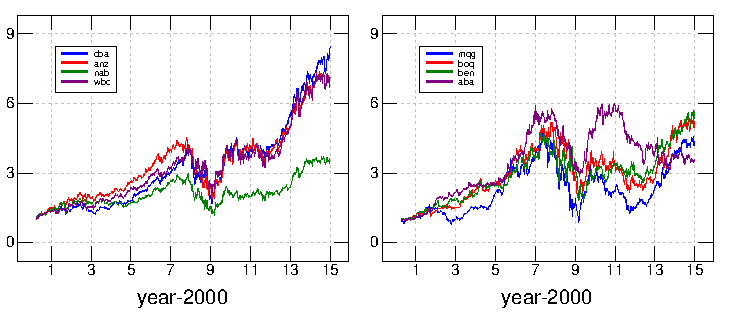
\includegraphics[width=10cm]{figures/prices.pdf}
\caption{Stock  prices of four major (left panel) and four minor (right panel) Australian banks from early 2000 through to the end of 2014.  Price series normalised to start at 1.}
\label{prices}
\end{center}
\end{figure}
}


\newcommand{\vareps}{\varepsilon}

\frame{\frametitle{Stress on Aust bank from market downturns}
\bi
\i  $S=dk(1-\e^{r-\ell})$ bank shortfall; $r$ is forward rate of return
\i  Stressor $\omega$ -- general stock market return
\i   \framebox{$f(S,\omega)$} from \framebox{$\delta_t\sim$ TARCH(1,1)-DCC}
\i  $\delta_t$ drives $r$ (monthly return) and $S$ (shortfall at end of month)
\bi
\i \framebox{$\delta_{t}=\mu+\sigma_{t}\eps_{t}$}  ...  $\eps_{t}\sim (0,1)$
\i \framebox{$ \sigma_{t+1}^2 = \omega+ \sigma^2_{t}\{\beta+(\alpha+\gamma \eps^-_{t})\eps_{t}^2\}$} ... volatility $\sigma_t$ is dynamic
\i $\eps^-_{t}\equiv I(\eps_{t}<0)=I(\delta_{t}<\mu)$
\ei 
\i  Similar model for daily \framebox{market} return
\i Correlation bank/market return from recursion -- \framebox{DCC}
$$
(Q_{t+1}-S) = \alpha (\eta_{t}\eta_{t}'-S) + \beta (Q_{t}-S)\cq \eta_{t}\equiv(\eps_{t},\eps_{mt})' .
$$
\i  Estimate unknown parameters -- quite a few -- use \framebox{R}
\bi
\i Model estimated to end of each month (2003 -- 2015)
\ei
\i  Project/simulate model forwards 1 month
\bi
\i  Use ``bootstrapped" $\eta_t$ in forward projection
\i  Use same ``bootstrapped" $\eps_{mt}$ for different joint models
\ei
\ei
}

\frame{\frametitle{CBA and market return}
\begin{figure}[htbp]
\begin{center}
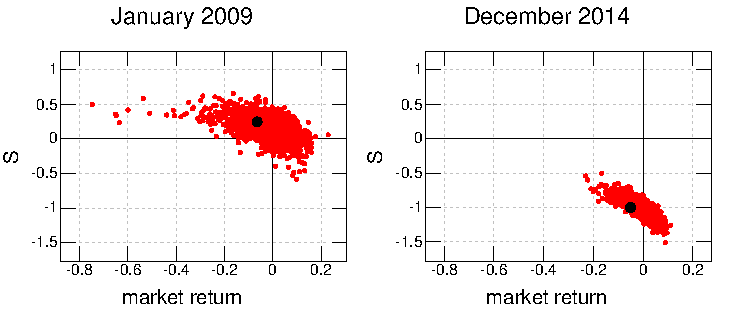
\includegraphics[width=9cm]{figures/figCBA.pdf}
\caption{Forecast bivariate distribution of one month rates of return   for CBA and the market rate of return}
\label{figCBA}
\end{center}
\end{figure}
\bi
\i  Daily model is ``cranked" forward 1 month
\i  No ``look ahead" bias -- use only past data relative to $t$
\i  Do same (ie estimate/project) at start of every month
\i  Bootstrapped errors:   error distribution ``like past"
\ei
}


\frame{\frametitle{Australian Banks: risks over time}
\begin{figure}[htbp]
\begin{center}
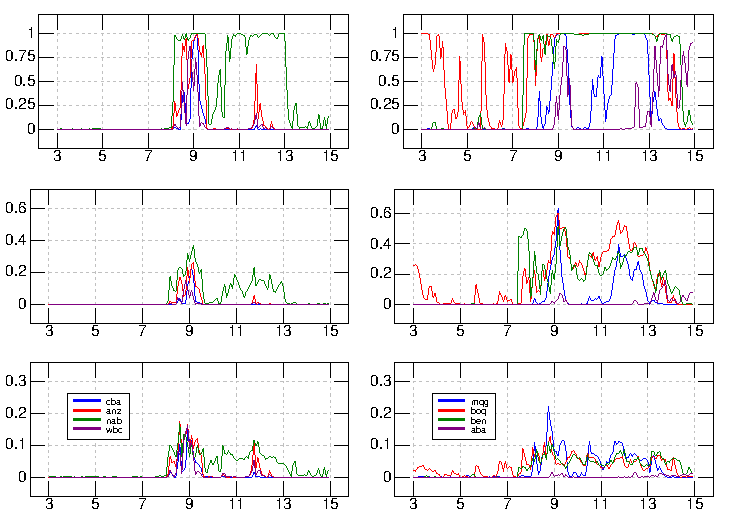
\includegraphics[width=8cm]{figures/default.pdf}
\caption{Forecast one month ahead  $\p(S>0)$ (top panels), BASRISK $\E(S^+)/(kd)$ (middle panels) and PSIRISK $\psi_{S^+}/(kd)$ 
(bottom panels) for  four major (left panel) and four minor (right panel)  banks 2003--2014.  Note different scale on bottom two rows of panels. $\psi$--risk is worst market outcome in 12 months.}\label{default}
\end{center}
\end{figure}
}

\frame{\frametitle{SRISK -- systemic risk}
\bi
\i Brownlees \& Engle (2015) define:
$$
\mathrm{SRISK} \equiv \sum_i\{\widetilde\E(S_i)\}^+ \cq 
\mathrm{SRISK}_i\equiv\frac{\{\widetilde\E(S_i)\}^+}{\mathrm{SRISK}}
$$
\bi 
\i $S_i \equiv kd_i\left(1-\e^{r_i-\ell_i}\right)$;  ``positive part of" is $^+$
\i stress is ``general market downturn greater than 10\%" 
\i  Computed at start of each month, looking 1 month forward
\i   SRISK$_i$ is \framebox{systemic risk} in firm $i$ 
\ei
\i Criticisms/Extensions of SRISK:
\bi
\i  Why not $\sum_i\widetilde\E(S_i^+)$: properties, alternatives 
\i  $\widetilde\E$ restrictive:  generalised here with $\psi$
\i  $\widetilde\E = \E + \cov$:  only cov  contains ``systemic" risk
\ei 
\i  Our definition incorporates all 3 adjustments and clarifies risk:
$$
\mathrm{BASRISK}\equiv \sum_i\E(S_i^+)\cq \mathrm{PSIRISK}\equiv \sum_i\cov(S_i^+,\psi) 
$$
\ei
}

\frame{\frametitle{Aggregate BASRISK and PSIRISK}
$$
\mathrm{BASRISK}\equiv \sum_i\E(S_i^+)\cq\mathrm{PSIRISK}\equiv \sum_i\cov(S_i^+,\psi)
$$
\bi
\i  components in  sums are BASRISK$_i$ and PSIRISK$_i$
\i  Risks additive eg PSIRISK$=\cov(\sum_iS_i^+,\psi)$
\i  \%PSIRISK in firm $i$ is $100\times\frac{\mathrm{PSIRISK}_i}{\mathrm{PSIRISK}}$
\i  Write $S_*=\sum_iS_i$ as the ``pooled" shortfall (pool $d$ and $w$) 
$$
\mathrm{BASRISK}_*\equiv \E(S_*^+)\cq \mathrm{PSIRISK}_*\equiv \cov(S_*^+,\psi)
$$
\i  $\mathrm{BASRISK}-\mathrm{BASRISK}_*=\E\left\{(\sum_iS_i^+)-(\sum_iS_i)^+\right\}\ge 0$
\i  $\mathrm{PSIRISK}-\mathrm{PSIRISK}_*=\cov\left\{(\sum_iS_i^+)-(\sum_iS_i)^+,\psi\right\}$ ?

\ei
}

\frame{\frametitle{BASRISK and PSIRISK at two dates}
 \begin{table}[ht]
\centering
\begin{threeparttable}
\tiny
\begin{tabular}{l|rrrr|rrrr}
\hline
&\multicolumn{4}{c|}{January 2009}&\multicolumn{4}{c}{November 2014}\\
\hline
   & Aloglev& Debt & BASRISK & PSIRISK  & Aloglev & Debt  & BASRISK & PSIRISK\\  
  \hline
CBA & 18.57 & 24.30 & 22.99 & 29.60 & -70.34 & 22.70 & 0.00 & 0.00 \\ 
  ANZ & 15.93 & 18.37 & 14.87 & 18.89 & -38.64 & 22.10 & 0.00 & 0.00 \\ 
  NAB & 31.97 & 25.50 & 39.98 & 19.41 & -12.45 & 25.61 & 50.52 & 67.13 \\ 
  WBC & -1.55 & 22.84 & 5.86 & 23.94 & -53.84 & 22.03 & 0.00 & 0.00 \\ 
  MQG & 41.22 & 5.75 & 11.02 & 5.46 & -46.10 & 4.33 & 0.17 & 0.12 \\ 
  BOQ & 63.30 & 1.32 & 3.55 & 0.99 & -17.05 & 1.33 & 0.80 & 1.34 \\ 
  BEN & 18.91 & 1.81 & 1.72 & 1.71 & -7.63 & 1.84 & 25.43 & 30.71 \\ 
  ABA & -8.12 & 0.10 & 0.00 & 0.00 & 9.22 & 0.07 & 23.07 & 0.71 \\ 
  \hline
  Total & 18.78 &  & 17.17 & 8.63 & -41.91 &   & 0.03 & 0.12 \\ 
  * (pooled) & 17.81 & 2.42 & 15.28 & 10.18 & -44.22 & 3.27 & 0.00 & 0.00 \\ \hline
\end{tabular}
\begin{tablenotes}
\item[]Response is $S_i^+$, the positive part of capital shortfall. PSIRISK is with respect to expected worst monthly market return  in 12 months.  Main body of table displays percentage contributions of each firm to total debt, BASRISK and PSIRISK.   ``Total" row displays debt weighted average of adjusted log--leverage, BASRISK and PSIRISK are per $100k\times$debt.    Pooled  displays   results with debt and equity pooled across banks: pooled debt is in \$$10^{11}$.  Pooled   BASRISK and PSIRISK are per $100k\times$debt.  
\end{tablenotes}
\end{threeparttable}
\end{table}
\normalsize
\bi
\i  PSIRISK:   worst {\bf monthly} market return  in 12 months
\bi
\i given \framebox{then current} {\bf daily}  return distribution
\ei
\i  PSIRISK-PSIRISK$_*$ measures absorbability
\i  Jan 2009:   PSIABS$<0$ ... non absorbable $\psi$--risk
\ei 
}

\frame{\frametitle{BASRISK and PSIRISK  over time}
\bi
\i  System risk: worst market outcome in 12 months
\begin{figure}[htbp]
\begin{center}
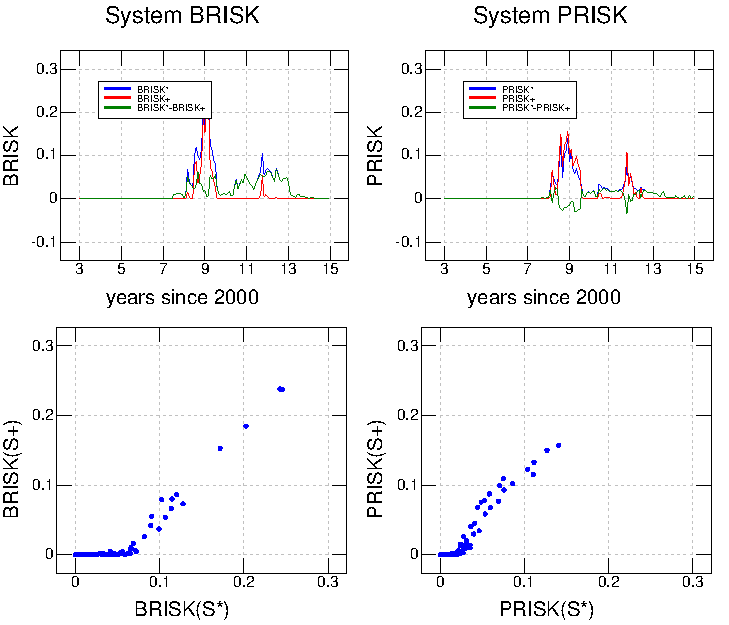
\includegraphics[height=4cm]{figures/muqs.pdf}
\end{center}
\end{figure}
\i Top panels 
\bi 
\i  Left panel BASABS=BASRISK$-$BASRISK$_*\ge 0$ 
\i  Right panel PSIABS=PSIRISK$-$PSIRISK$_*\ngeqslant 0$
\i  PSIRISK can be ``contagious"
\ei
\i  Bottom panels:
\bi
\i  BASRISK (x--axis) versus  BASRISK$_*$  ... ditto for PSIRISK
\i  Contagion effects builds up ``later"
\ei   
\ei
}

\newcommand{\Ax}{{\cal A}}
\frame{\frametitle{Formalising risk weighted assets methodology}
Future shortfall in terms of assets $a\equiv d+w=\sum_ja_j$
$$
S\equiv  d-\alpha\Ax(\e^{r_j})\cq \alpha\equiv(1-k)a\cq \Ax(\e^{r_j})\equiv \sum_j\frac{a_j}{a}\e^{r_j}
$$
\bi
\i  $r_j$ is (uncertain) log--return on assets $a_j$
\i $\E(S)=d-\alpha\E\{\Ax(\e^{r_j})\}=d-\alpha\Ax\{\E(\e^{r_j})\}$
\i  Risk weighting methodology:  replace $\frac{a_j}{a}$ weights by $
\frac{a_j}{a\sigma_j}$
\bi
\i   How to determine the weights $\sigma_j$?
\ei
\i PSIRISK approach: replace $\E$ by $\widetilde\E$ using suitable $\psi$
\bi
\i $\psi_S=\widetilde\E(S)-\E(S)= -\alpha\cov\left\{\Ax(\e^{r_j}),\psi\right\}=-\alpha\Ax\{\cov(\e^{r_j},\psi)\}$
\i $\psi_S\approx -\alpha\Ax\{\cov(r_j),\psi\}$ since $\e^{r_j}\approx 1+r_j$
\i $\cov(r_j,\psi)\ll0$ implies  $a_j$ is  discounted
\ei
\i  Modelling
\bi
\i  Simulate from $f(r_j,\psi)=f(\psi)f(r_j|\psi)$ eg GARCH-DCC
$$
 \mathrm{BASRISK}\approx d-\alpha\Ax\{\E(r_j)\}\cq  \mathrm{PSIRISK}\approx -\alpha\Ax\left\{\cov(r_j,\psi)\right\}
$$
\i Alternatively use $f\{\Ax(r_j),\psi\}=f(\psi)f\{\Ax(r_j)|\psi\}$
\i if using eg $S^+$  then calculate $\psi_S$ via $\widetilde\E(S^+)-\E(S^+)$
\ei
\ei
}

\frame{\frametitle{Conclusions}
\bi
\i Have presented a consistent methodology for stress testing
\i Formalises intuitive approach to stress testing
\i Requires:
\bi
\i  An appropriate response subject to potential stress
\i  Scenario space
\i  Natural scenario probabilities
\i  Stress function defined on scenario space
\i A joint statistical model for the response and scenarios
\ei
\i Frameworks leads to natural definitions of
\bi
\i BASRISK -- baseline risk
\i PSIRISK -- risk due to assumed stress
\ei
\i BASRISK and PSIRISK aggregate additively
\i Concepts provide framework for defining risk diversifiability and contagion
\ei
}

\end{document}
